\section{Service-oriented Architecture}

\begin{frame}{Service-oriented Architecture}
    \begin{itemize}
        \item Bisher: Eng gekoppelte Funktionalitäten
        \item Jetzt: Lose Kopplung von Funktionalitäten durch Kapselung als Dienst
        \item Ziel Service-oriented Architecture (SOA): Wiederwendung von Funktionalitäten
    \end{itemize}
\end{frame}

\begin{frame}{Service-oriented Architecture: Komponenten}
    \begin{itemize}
        \item Service Provider: Stellt spezifischen Dienst bereit
        \item Service Consumer: Nutzt bereitgestellten Dienst
        \item Broker: Vermittler, der Kommunikation zwischen Consumer und Provider regelt
        \item Service Registry: Sammlung von Metadaten zu Services und deren Provider
    \end{itemize}
\end{frame}

\begin{frame}{Service-oriented Architecture: Struktur}
    \begin{figure}[!h]
        \centering
        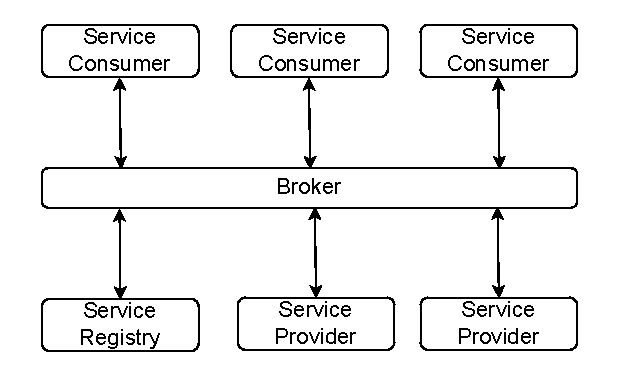
\includegraphics[scale=0.80]{imglib/soa/soa}
        \caption{Aufbau der Service-oriented Architecture}
        \label{fig:soa}
    \end{figure}
\end{frame}

\begin{frame}{Service-oriented Architecture: Beispiel E-Commerce I}
    \begin{itemize}
        \item \texttt{OrderService}: Dienst für Verwaltung von Bestellungen
        \item \texttt{PaymentService}: Dienst für die Abwicklung von Zahlungen (Service von PayPal, \ldots)
        \item \texttt{ShipmentService}: Dienst für den Versand (Service von DHL, \ldots)
    \end{itemize}
\end{frame}

\begin{frame}{Service-oriented Architecture: Beispiel E-Commerce II}
    \begin{figure}[!h]
        \centering
        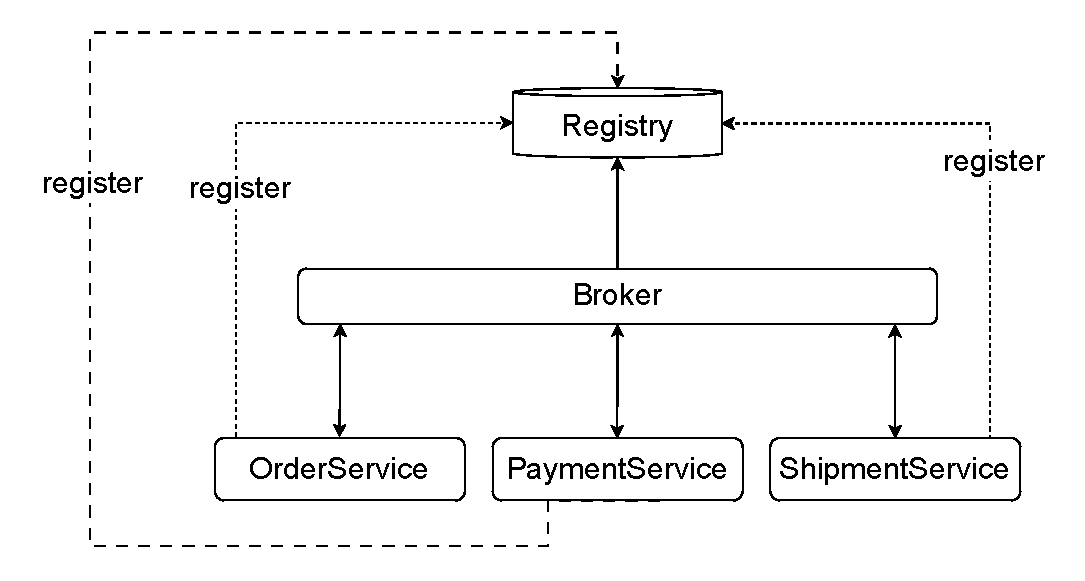
\includegraphics[scale=0.50]{imglib/soa/soa-example}
        \caption{E-Commerce-Beispiel mit Service-oriented Architecture}
        \label{fig:soaecommerce}
    \end{figure}
\end{frame}

\begin{frame}{Service-oriented Architecture: Agilität}
    \begin{itemize}
        \item Wie bei modularem Monolithen: Lose Kopplung $\Rightarrow$ kleine autonome Teams
        \item Aber zusätzlich: Deployment in Teams $\Rightarrow$ kürzere Iterationen \& häufigere Auslieferung
        \item Dadurch: Flexibler gegenüber wechselnden Anforderungen
        \item Zeit- und Kosteneinsparungen durch Wiederverwendung von Diensten
        \item Eigenständige Dienste ermöglichen horizontale Skalierung
        \item Aber: Langfristig Abhängigkeiten zwischen Diensten, besonders für grob-granulare Dienste
    \end{itemize}
\end{frame}